\documentclass{article}
\usepackage[utf8]{inputenc}
\usepackage[dutch]{varioref}
\usepackage[autostyle]{csquotes} 
\usepackage[dutch]{babel}
\usepackage{pdfpages}

\title{Stageverslag}
\author{\mbox{Pieter-Jan} Robrecht}
\date{Maart 2016}
\usepackage{natbib}
\usepackage{graphicx}

\begin{document}

%\maketitle
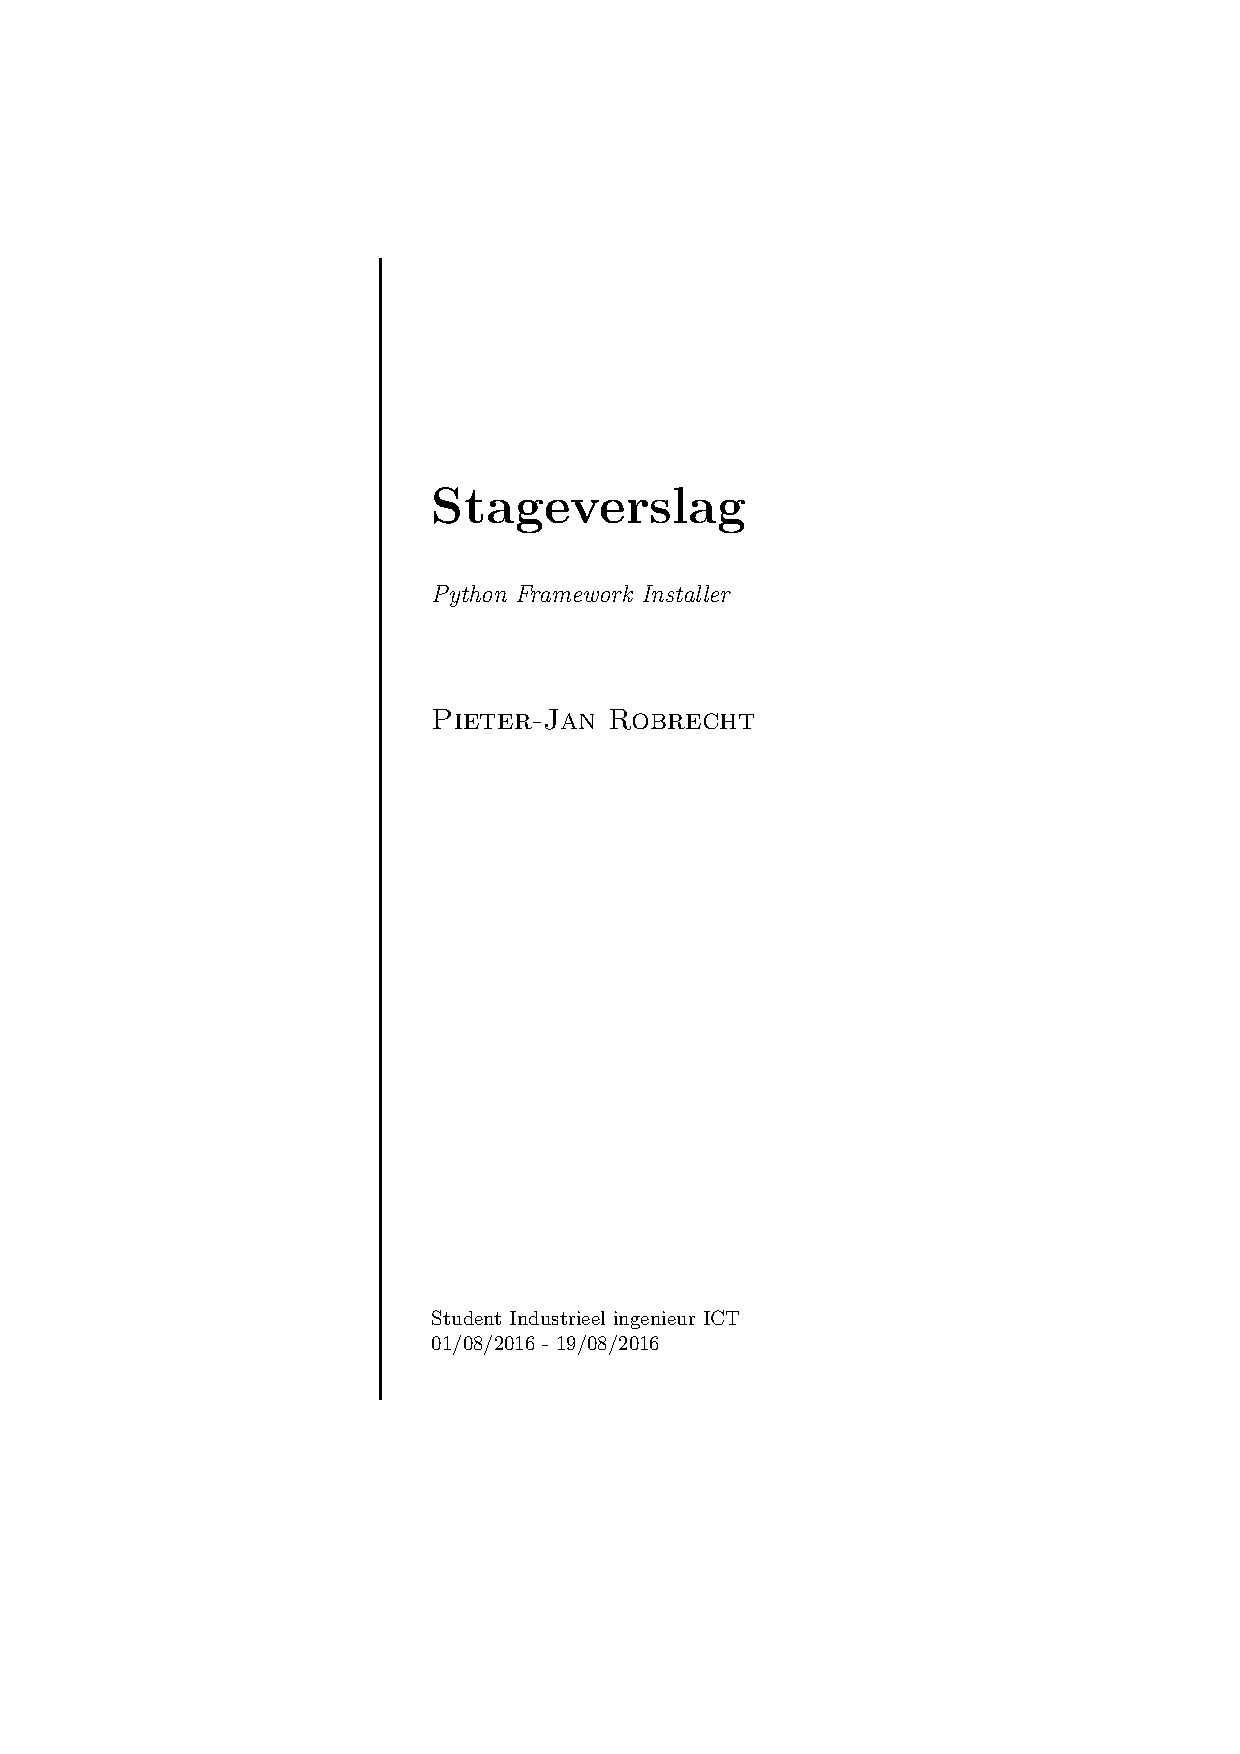
\includepdf{titel/titelstage.pdf}

%Volgende lijn is om de titelpagina geen paginanummer te geven
\clearpage
\setcounter{page}{1}
\tableofcontents
\clearpage

\section{Inleiding}
In het kader van mijn masterproef was het mogelijk om bij Televic Rail een stage te lopen tijdens de zomer. 
Gedurende deze stage heb ik mijn masterproef voorbereid en onderzoek gedaan naar de verschillende mogelijkheden die er zijn voor het uitvoeren van mijn opdracht.
De opdracht die voltooid moet worden is de volgende:
\begin{displayquote}
Televic Rail heeft een Python test framework ontworpen. 
Dit framework werd oorspronkelijk gebruikt om gebruikt te worden op een volledig uitgeruste testtoren, maar het framework werd aangepast zodanig dat het onafhankelijk van de testtoren gebruikt kan worden.
Aangezien het framework gebruik maakt van verschillende niet-standaard Python bibliotheken, is het installeren van het framework op een nieuw systeem een hele klus.
Het doel is dan ook het maken van een installer en een updater waarmee dit proces kan worden vergemakkelijkt zodanig dat er zo min mogelijk interactie van de gebruiker moet zijn.
\end{displayquote}
Tijdens de duur van de stage werden de verschillende implementatie manieren onderzocht en werd er een algemene architectuur voor de installer-updater uitgedacht.
In wat volgt wordt er beschreven welke stappen er werden ondernomen om het probleem onder te verdelen in enkele logische stappen en hoe deze problemen dan werden opgelost. 

\section{Analyse van het probleem}
Tijdens het bespreken van het probleem werd het al snel duidelijk dat er verschillende scenario's zijn waarin het framework gaat gebruikt moeten worden. Het framework zal gebruikt moeten worden als een standalone programma op een laptop of desktop maar het zal ook moeten draaien op de verschillende testtorens. Beide omgevingen zullen Windows gebruiken als besturingssysteem. Er zullen dus geen grote veranderingen moeten worden aangebracht in het maken van de installer aangezien beide omgevingen overweg kunnen met een .exe bestand. Uiteraard moet er rekening worden gehouden met de toekomst. Het framework zal in de nabije toekomst worden aangepast zodanig dat het mogelijks op een raspberry pi kan draaien. Dit zou wel voor verschillende problemen kunnen zorgen aangezien een raspberry pi een linux distributie zal gebruiken als zijn besturingssysteem. 

\section{Oplossingen}

\end{document}